%导言区
\documentclass[10]{article}

\usepackage{ctex}
\usepackage{graphicx}
\usepackage {subfigure}
\usepackage{float}
\usepackage{amsmath}
\usepackage{amssymb}

\bibliographystyle{plain}
\title{Rgression}
\author{Prevalenter}
\date{\today}
\graphicspath{{img/}}
\begin{document}
	\maketitle
	%\chapter{绪论}
	\section{test}
	%字体族设置(罗马字体 无称线字体 打字机字体)
	\subsection{font test}
	\textrm{Roman Faily}
	
	\textsf{Sans serif Family}
	
	\texttt{Typewriter Family}
	%hello,\LaTeXe
	Let $f(x)$ be defined by the formula
	$$f(x)=3x^2+x-1$$
	which is a polynomial of degree 2.
	
	测试下中文
	
	\section{插入图片}
	Figure \ref{Fig.lable} has two sub figures, fig. \ref{Fig.sub.1} is the travel demand of driving auto, and fig. \ref{Fig.sub.2} is the travel demand of park-and-ride.
	
	\begin{figure}[H]
		\centering
		\subfigure[SubfigureCaption]{
		\label{Fig.sub.1}
		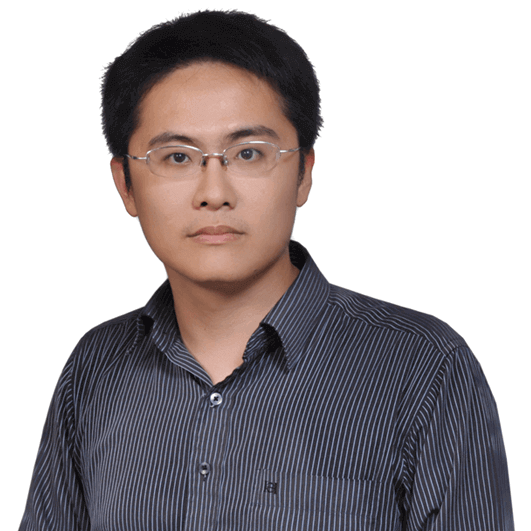
\includegraphics[width=0.4\textwidth]{lee}}
		\subfigure[SubfigureCaption]{
		\label{Fig.sub.2}
		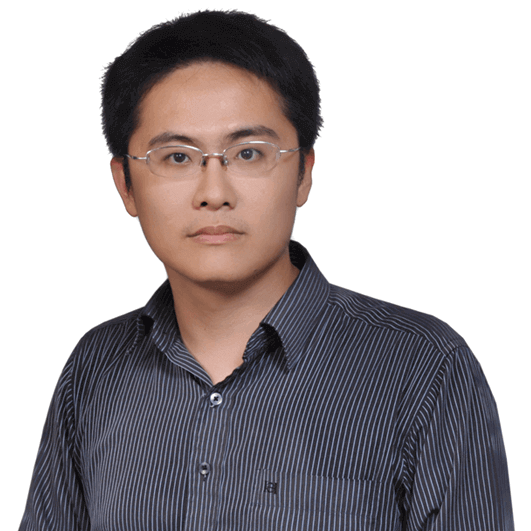
\includegraphics[width=0.4\textwidth]{lee}}
		\caption{MainfigureCaption}
		\label{Fig.lable}
	 %\caption{Visual comparison samples between the original saliency map and enhanced saliency map by centre-bias and human visual acuity.}
		\label{fig:visual_smap}
	\end{figure}

	\section{表格}
	表\ref{table-score}所表示的是期末的成绩单
	\begin{table}[h]
	\centering
	\caption{成绩单}\label{table-score}
		\begin{tabular}{|l| c| c| c|p{1.5cm} |}
			\hline
			姓名 & 语文 & 数学 & 外语 & 备注 \\
			\hline
			张三 & 语文 & 数学 & 外语 & 备注 \\
			\hline
			李四 & 语文 & 数学 & 外语 & 备注 \\
			\hline
		\end{tabular}
	\end{table}

	\section{数学公式}
	勾股定理公式见公式\ref{equation1}:
	\begin{equation}
		a^{2}=b^{2}+c^{2}\label{equation1}
	\end{equation}
	
	如:
	\begin{equation}
	5^{2}=3^{2}+4^{2}\label{equation2}
	\end{equation}
	
	\section{矩阵}
	使用matrix环境输入矩阵
	$$\begin{pmatrix}
		0 & 10 & 10 & 1\\
		1 & 00 & 10 & 1\\
		0 & 10 & 10 & 1\\
		1 & 00 & 10 & 1
	\end{pmatrix}
	\begin{pmatrix}
	0 & 10 & 10 & 1\\
	1 & 00 & 10 & 1\\
	0 & 10 & 10 & 1\\
	1 & 00 & 10 & 1
	\end{pmatrix}$$
	\[ \mathbf{X} = \left( \begin{array}{cccc} x_{11} & x_{12} & \ldots & x_{1n}\\ x_{21} & x_{22} & \ldots & x_{2n}\\ \vdots & \vdots & \ddots & \vdots\\ x_{n1} & x_{n2} & \ldots & x_{nn}\\ \end{array} \right) \]
	
	\section{多行公式}
	
	带编号的公式如:
	\begin{gather}
		3+4=5\\
		a+b=c
	\end{gather}
	不带符号的公式如:
	\begin{gather*}
	3+4=5\\
	a+b=c\\
	\end{gather*}
	多行不等式有:
	\begin{equation}
		\begin{split}
		\cos 2x &= \cos^2 x -\sin^2 x \\
		&=2\cos^2 x - 1
		\end{split}
	\end{equation}
	花括号大公式有:
	\begin{equation}
		D(x)=\begin{cases}
		1,&\text{如果} x \in \mathbb{Q};\\
		0,&\text{如果} x \in \mathbb{R}\setminus\mathbb{Q};
		\end{cases}
	\end{equation}
	这是一个文件的引用\cite{patashnik1988designing}
	
	\bibliography{test}
\end{document}